% Created 2019-03-19 Tue 16:18
\documentclass[presentation]{beamer}
\usepackage[utf8]{inputenc}
\usepackage[T1]{fontenc}
\usepackage{fixltx2e}
\usepackage{graphicx}
\usepackage{longtable}
\usepackage{float}
\usepackage{wrapfig}
\usepackage{rotating}
\usepackage[normalem]{ulem}
\usepackage{amsmath}
\usepackage{textcomp}
\usepackage{marvosym}
\usepackage{wasysym}
\usepackage{amssymb}
\usepackage{hyperref}
\tolerance=1000
\usetheme{default}
\author{Jonatan Ahumada Fernández}
\date{\today}
\title{Sumas de Riemann e integrales}
\hypersetup{
  pdfkeywords={},
  pdfsubject={},
  pdfcreator={Emacs 25.3.1 (Org mode 8.2.10)}}
\begin{document}

\maketitle
\begin{frame}{Outline}
\begin{itemize}
\item sumatorias y propiedades
\item ¿de qué nos sirven las sumatorias al integrar?
\item ejemplo de una integral por sumas 
\end{itemize}
\end{frame}


\begin{frame}[label=sec-1]{Video1 : notación sigma y sus propiedades:}
\begin{block}{Sintaxis}
Consideremos: 

\[\sum_{i=k}^{n}a_{i} = a_{k} + a_{k + 1} + \dots + a_{n}\]

\begin{itemize}
\item $\Sigma$ = notación sigma
\item k = límite inferior
\item n = límite superior
\item i = índice de la sumatoria
\item a$_{\text{i}}$ = formas que toman los sumandos
\end{itemize}
\end{block}

\begin{block}{Tener en cuenta}
\begin{itemize}
\item es la representación de una suma
\item cantidades pueden ser finitas o infinitas
\end{itemize}
\end{block}
\end{frame}

\begin{frame}[label=sec-2]{Propiedades}
Las propiedades van a permitir manipular las sumatorias con mayor facilidad.
Por ejemplo, expresar una sumatoria en términos de otras más sencillas.

Las propiedades enunciadas en el video son:
\end{frame}

\begin{frame}[label=sec-3]{1) Número de términos de una sumatoria}
Para

\[\sum_{i=k}^{n}a_{i} = a_{k} + a_{k + 1} + \dots + a_{n}\]


\[ Número\ de\ términos  = n - k + 1  \]
\begin{block}{Ejemplo}
\[\sum_{i=3}^{7}i = 3 + 4 + 5 + 6 + 7\] 
\end{block}
\end{frame}




\begin{frame}[label=sec-4]{2) Para sumas y diferencias de dos o más variables:}
\begin{itemize}
\item Se puede reescribir la sumatoria como varias sumatorias distintas
\end{itemize}


\[\sum_{i=n}^{k}(a_{i} + b_{i} - c_{i}) = \sum_{i=n}^{k}a_{i} + \sum_{i=n}^{k} b_{i} - \sum_{i=n}^{k} c_{i} \] 
\end{frame}


\begin{frame}[label=sec-5]{3) Sumatoria de una constante:}
\begin{itemize}
\item Se multiplica la constante por el numero de términos de la sumatoria
\[\sum_{i=n}^{k} c = c * número\ de\ términos \]
\end{itemize}
\end{frame}

\begin{frame}[label=sec-6]{Ejemplo}
\[\sum_{i=2}^{8} 3 = 3 + 3 + 3 + 3 + 3 + 3 + 3\] 
\[\sum_{i=2}^{8} 3 = 3 * 7 \] 

No confundir con: 
 \[\sum_{i=2}^{8} i + 3  \]

\begin{itemize}
\item aquí sí está en función de una variable, no es constante
\end{itemize}
\end{frame}

\begin{frame}[label=sec-7]{4) Una sumatoria se puede descomponer en dos o más sumatorias parciales}
\[\sum_{i=1}^{k}x_{i} = \sum_{i=1}^{n}x_{i} + \sum_{i=n+1}^{k} x_{i} \] 
\end{frame}

\begin{frame}[label=sec-8]{5) Sumatoria de una constante y una o más variables}
\[\sum_{i=1}^{n}(ax_{i} \pm by_{i}) = a\sum_{i=1}^{n}x_{i} \pm b\sum_{i=1}^{n} y_{i} \]

\begin{itemize}
\item Mezcla de dos propiedades anteriores
\end{itemize}
\end{frame}

\begin{frame}[label=sec-9]{Ejemplo}
\begin{block}{¿Cuánto da esto?}
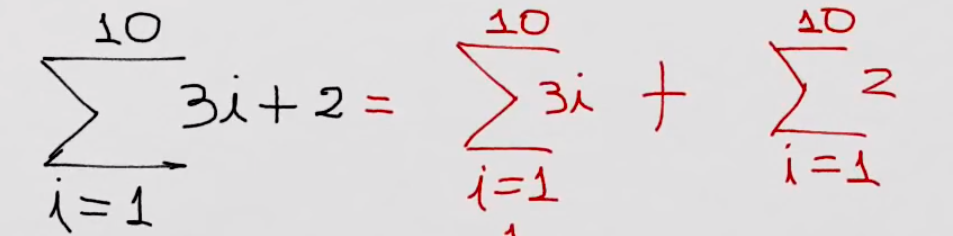
\includegraphics[width=.9\linewidth]{./ejercicio_desc.png}

\begin{itemize}
\item recordar \(Sn = \frac{(t1 + t2)}{2} * (número\ de\ términos)\)
\end{itemize}
\begin{block}{solución}
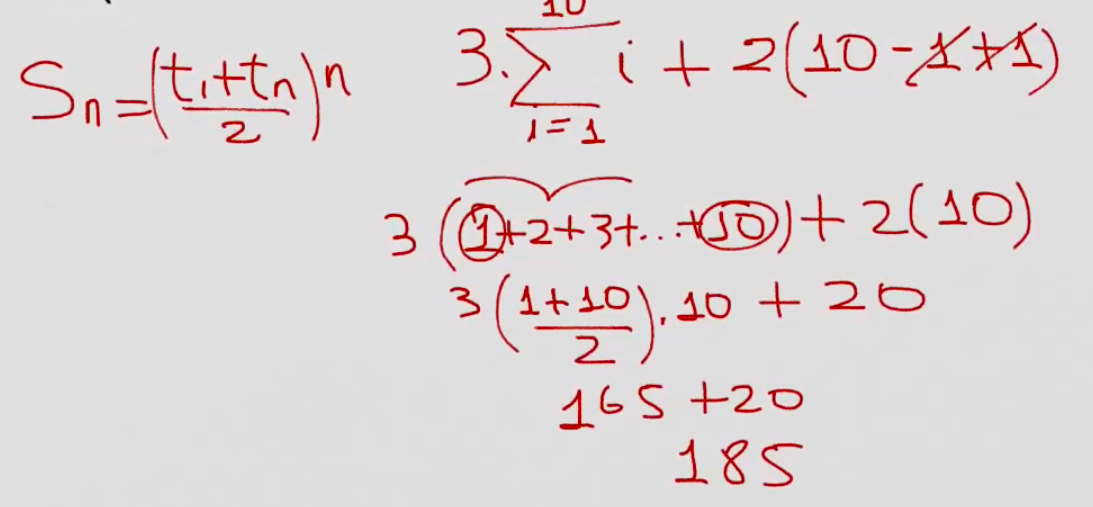
\includegraphics[width=.9\linewidth]{./ejercicio_desc2.png}
\end{block}
\end{block}

\begin{block}{Conclusión (combinación de todas las propiedades}
\begin{block}{¿Cuánto da esto?}
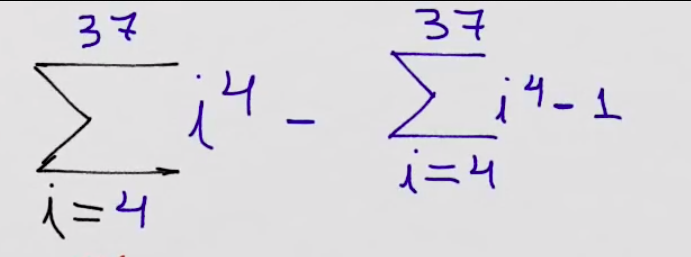
\includegraphics[width=.9\linewidth]{./ej_conclusion.png}
\end{block}

\begin{block}{Solucion}
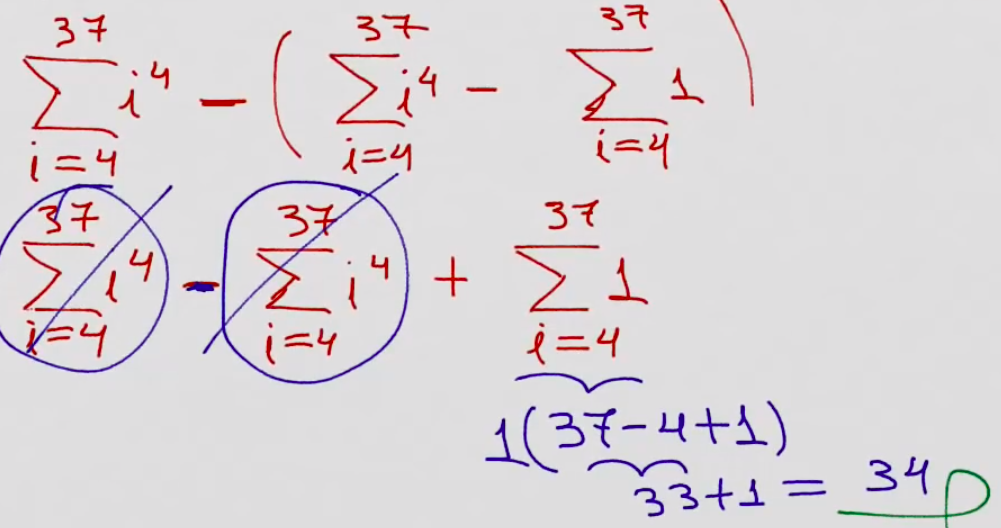
\includegraphics[width=.9\linewidth]{./ej_conclusion2.png}
\end{block}
\end{block}
\end{frame}


\begin{frame}[label=sec-10]{Video 2:}
Gráficamente, la integral describe el área bajo la curva. 
Por lo tanto, puede ser escrita:
\begin{block}{Una aproximación}
\[A \approx \sum_{i=1}^{n}f(x_{i})  \Delta x \]
\end{block}

\begin{block}{Una igualdad}
\[A =  \lim_{n\to\infty} \sum_{i=1}^{n}f(x_{i})  \Delta x \]
\end{block}

\begin{block}{¿Qué elementos de la interpretación geométrica correponden a \(f(x_{y})\) y \(\Delta x\)?}
\(f(x_{i}) =\ altura  \)
\(\Delta x =\ ancho \)
\end{block}
\end{frame}



\begin{frame}[label=sec-11]{Video  3: resolver una integral paso a paso}
\begin{block}{Evalúe la suma de Riemann para}
\[f(x) = x^3 - 6x\]

tomando los puntos extremos de la derecha con: 
\(a = 0\), \(b = 3\) y \(n = 6\)
\end{block}

\begin{block}{Entonces:}
\begin{enumerate}
\item lo expresamos como integral
\item lo expresamos como suma de Riemann
\end{enumerate}

\[\int_{a}^{b} f(x)dx = \lim_{n\to\infty} \sum_{i=1}^{n}f(x_{i})  \Delta x \]

y sabemos que

\[\Delta x = \frac{b - a}{n}\]
\end{block}
\end{frame}

\begin{frame}[label=sec-12]{Si evaluamos:}
\[\Delta x = \frac{3 - 0}{6} = \frac{3}{6} = 0.5\]

Para este ejercicio en particular, nos dan la condición de que \(n = 6\). Son 6 particiones únicamente, no 
tienden a infinito. 
\[\int_{0}^{3} f(x)dx = \sum_{i=1}^{6}f(x_{i}) * \Delta x \]
\end{frame}

\begin{frame}[label=sec-13]{evaluamos cada una de los rectángulos}
Como el delta nos dio 0.5

\begin{equation}
\begin{split}
x_{1} &= 0.5 \\
x_{2} &= 1.0 \\
x_{3} &= 1.5 \\
x_{4} &= 2.0 \\
x_{5} &= 2.5 \\
x_{6} &=  3.0
\end{split}
\end{equation}
\end{frame}

\begin{frame}[label=sec-14]{}
Entonces, si evaluamos \(f(x) = x^3 - 6x\) 
\begin{equation}
\begin{split}
 f(0.5) = (0.5)^3 - 6(0.5)  &= -2.875 \\
 f(1.0) = (1.0)^3 - 6(1.0)  &= -5 \\
 f(1.5) = (1.5)^3 - 6(1.5) &= -5.625 \\
 f(2.0) = (2.0)^3 - 6(2.0) &= -4 \\
 f(2.5) = (2.5)^3 - 6(2.5)  &= 0.625 \\
 f(3.0) = (3.0)^3 - 6(3.0)  &=  9
\end{split}
\end{equation}

Ahora sólo nos queda reemplazar estos valores en la sumatoria. 
Recordemos las propiedades de la sumatoria y nos queda: 

\[\sum_{i=1}^{6}f(x_{i}) * \Delta x = (-2.87 - 5 - 5.625 - 4 + 0.625 + 9)(0.5) \]


\[ \approx  3.9375 \]

\begin{block}{¿Por qué da un valor negativo?}
Porque la curva está por debajo del eje de las x. 
\end{block}
\end{frame}

\begin{frame}[label=sec-15]{¿Cómo se dibujan los rectángulos?}
En el ejemplo anterior cada valor marcaba su punta del lado derecho. 
\end{frame}

\begin{frame}[label=sec-16]{}
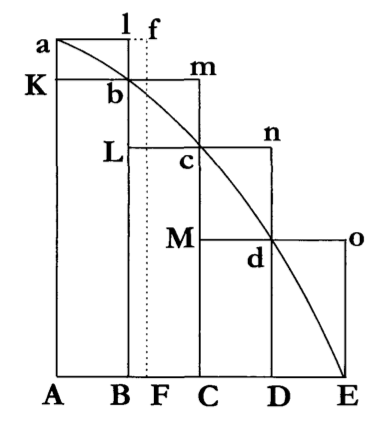
\includegraphics[width=.9\linewidth]{./puntos_extremos.png}
\end{frame}


\begin{frame}[label=sec-17]{Gracias..}
\end{frame}
% Emacs 25.3.1 (Org mode 8.2.10)
\end{document}